\section{Performance Evaluation}


\subsection{Implementation}
We implement \ours{} in \texttt{FEMU}, an open-source SSD development
framework~\cite{li2018case}. 
Fig.~\ref{fig_dawid_archi} shows the overall architecture of \ours{} SSD and
its internal data structures. 

To realize this design,  
\ours{} maintains two data structures: first, \textit{a zero-cost list}  
that holds the write requests whose mapping entry is already in a dirty translation page,  
and second, \textit{a max binary heap} that maintains the indexes to translation pages 
sorted by the number of buffered user write requests associated with that page.  
% We term this policy Least Increase of Dirtiness (LID) scheduling. 
When there is sufficient bandwidth at underlying NAND flash subsystem for writes,  
\ours{} first flushes user data from the  zero-cost list, 
and then persists the dirty translation pages as ordered by the max binary heap.  
By doing so, each user write minimizes the number of eventual translation page write,  
and each translation page write maximizes the number of persisted mapping entries. 

\begin{figure}[t]
    \centering{}
	\subfloat[Architecture] { 
    	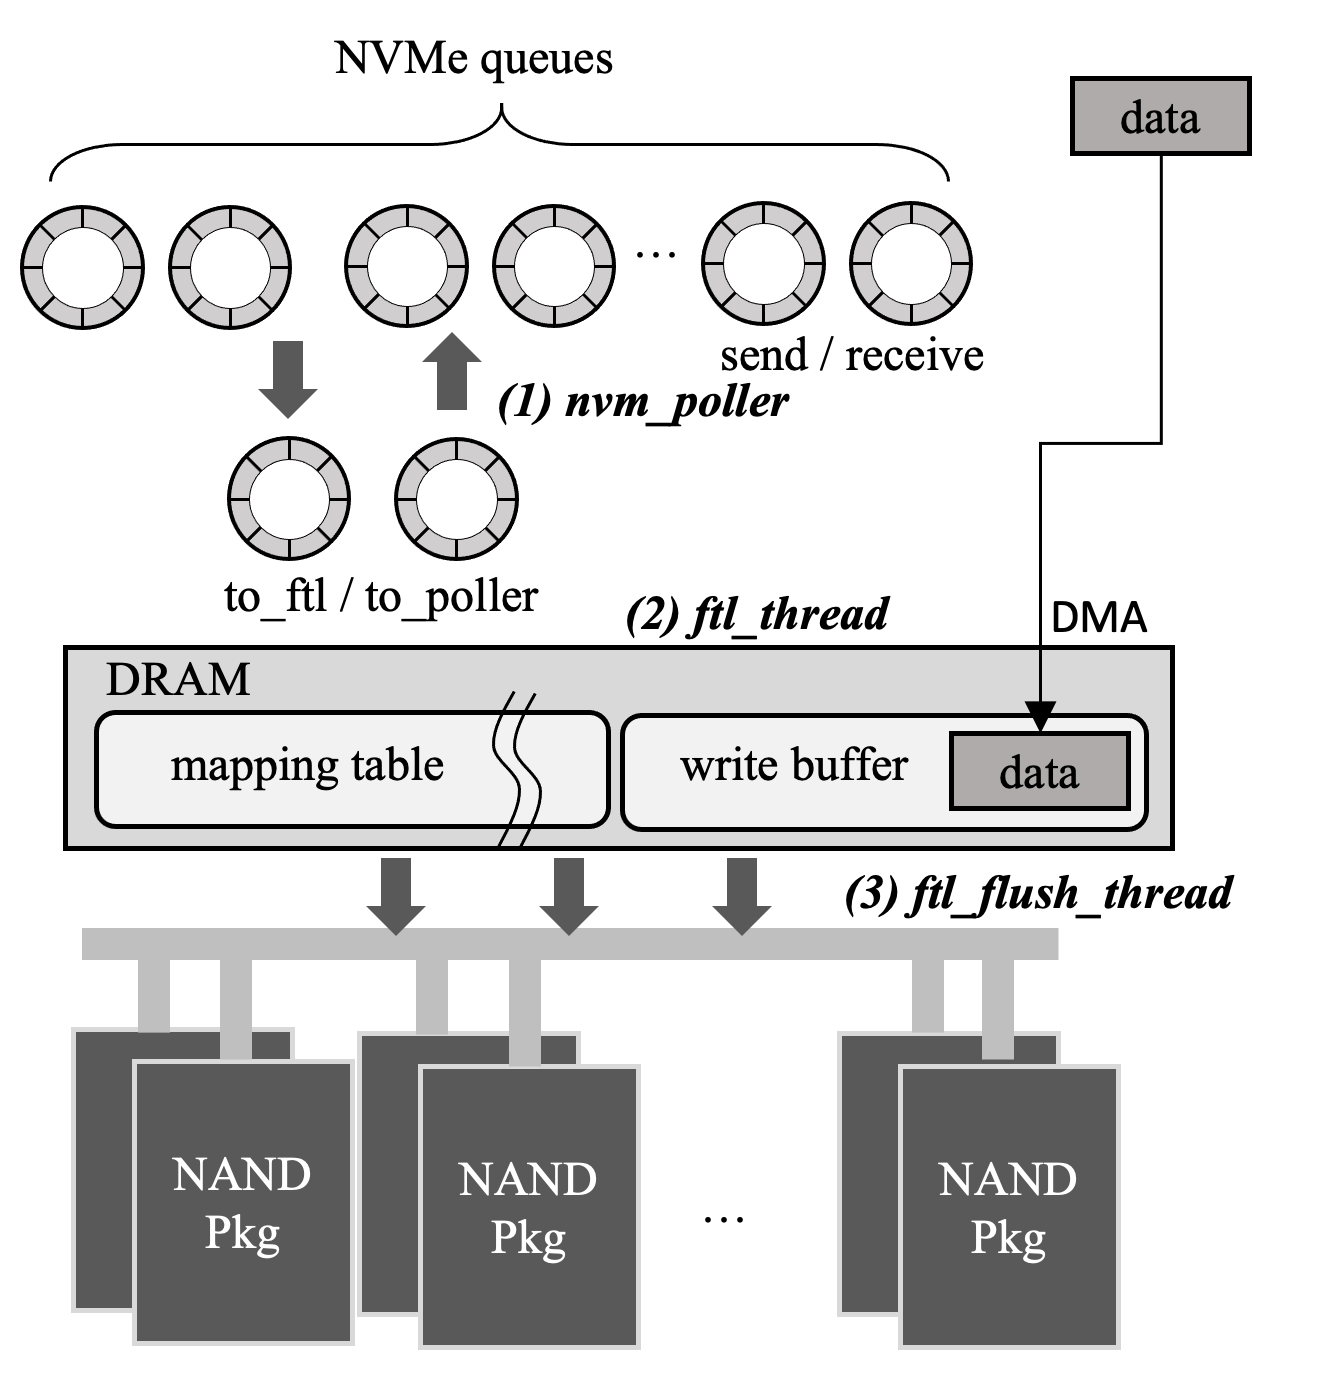
\includegraphics[width=0.3\textwidth]{figure/dawid_ssd_archi_new.eps}
	} \\
	\subfloat[Data structures for FTL]{ 
    	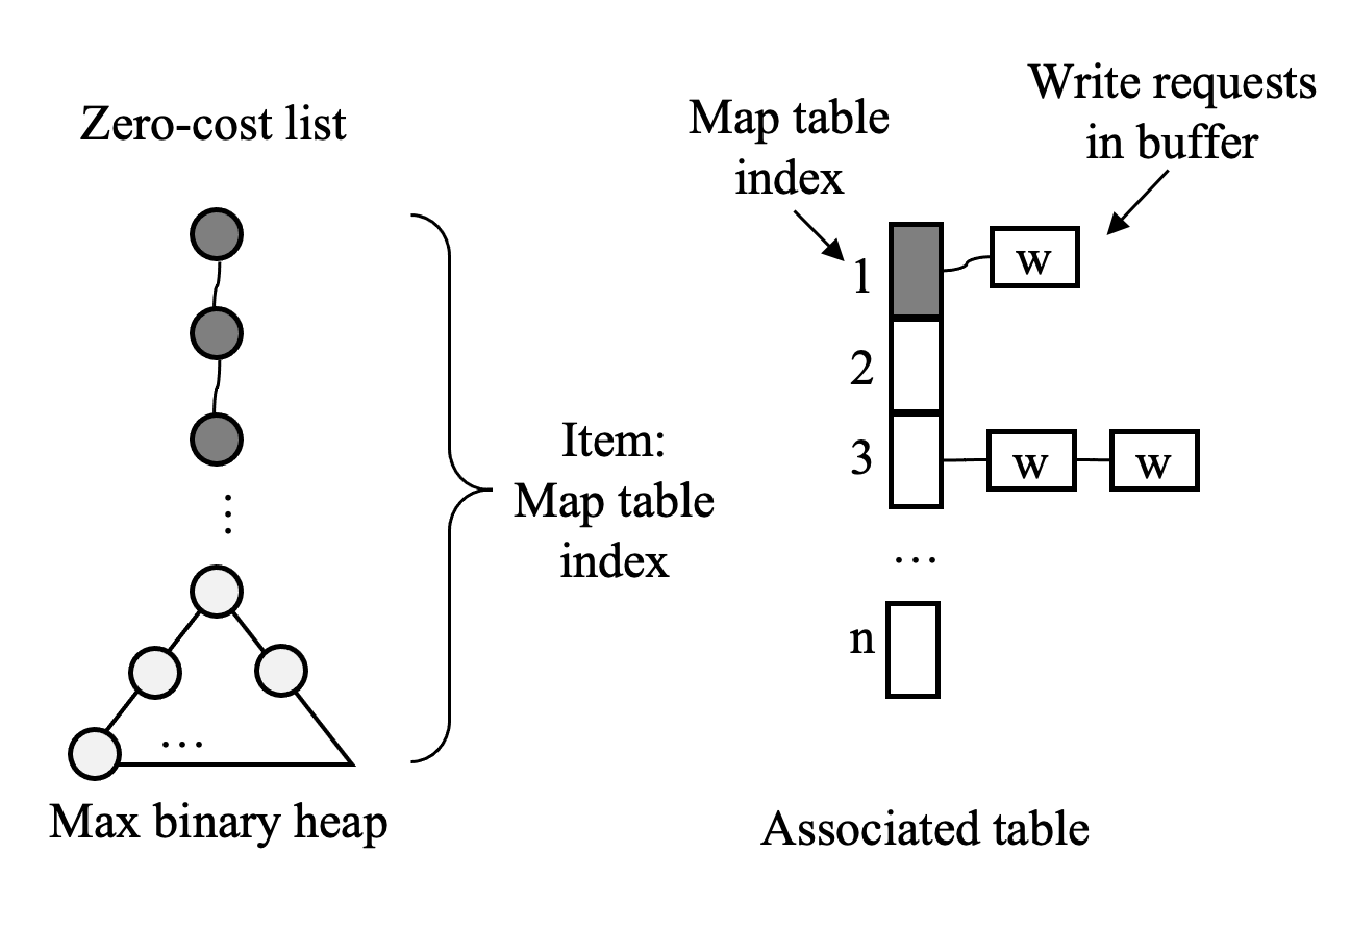
\includegraphics[width=0.4\textwidth]{figure/dawid_ds.eps}
	}

    %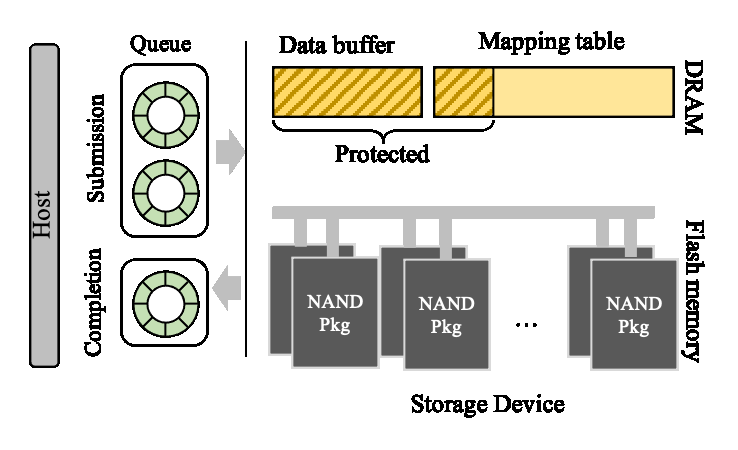
\includegraphics[width=0.4\textwidth]{figure/dawid_ssd_archi.eps}
    \caption{\textbf{Dawid-SSD.Architecturep}}
    \label{fig_dawid_archi}
\end{figure}






\begin{figure*}[t]
    \centering{}
	\subfloat[Sequential] { 
	    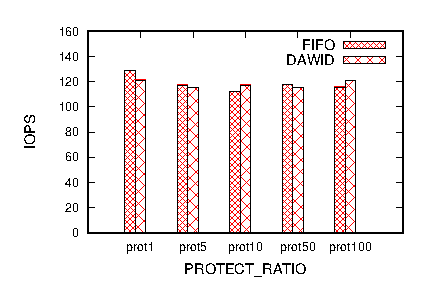
\includegraphics[width=0.3\textwidth]{expr/micro_220517/perf/SEQ/perf_SEQ.eps}
	} 
	\subfloat[Random] { 
	    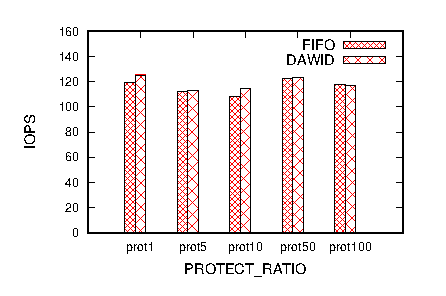
\includegraphics[width=0.3\textwidth]{expr/micro_220517/perf/RAND/perf_RAND.eps}
	} 
	\subfloat[JESD] { 
	    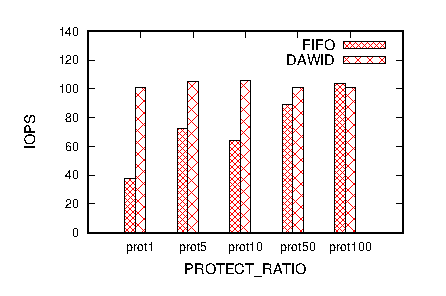
\includegraphics[width=0.3\textwidth]{expr/micro_220517/perf/JESD/perf_JESD.eps}
	}
    \caption{\textbf{IOPS}}
\end{figure*} 


\iffalse
\begin{figure*}[t]
	\includegraphics[width=0.9\textwidth]{expr/micro_220517/wt/result/total.rslt.eps}
    \caption{\textbf{Write Traffic}}
\end{figure*} 
\fi


\begin{figure*}[t]
    \centering{}
	\subfloat[Sequential] { 
	    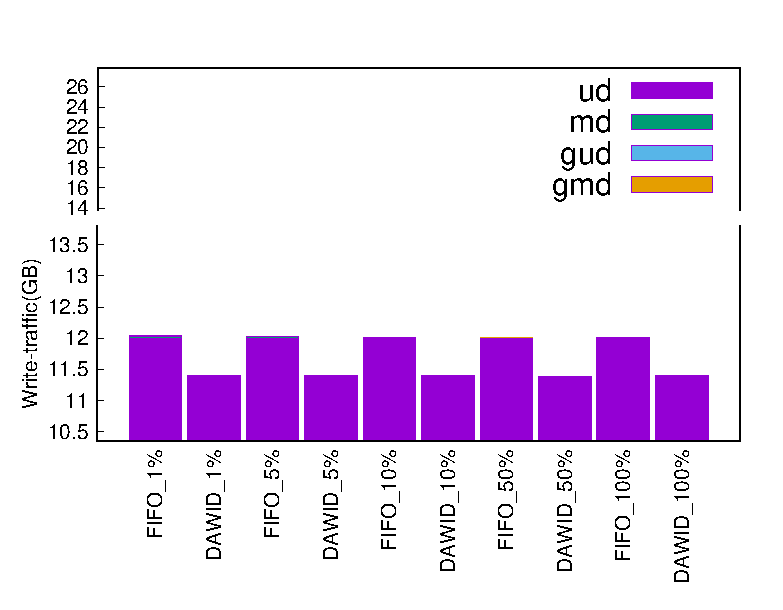
\includegraphics[width=0.3\textwidth]{expr/micro_220517/wt/result/SEQ.eps}
	} 
	\subfloat[Random] { 
	    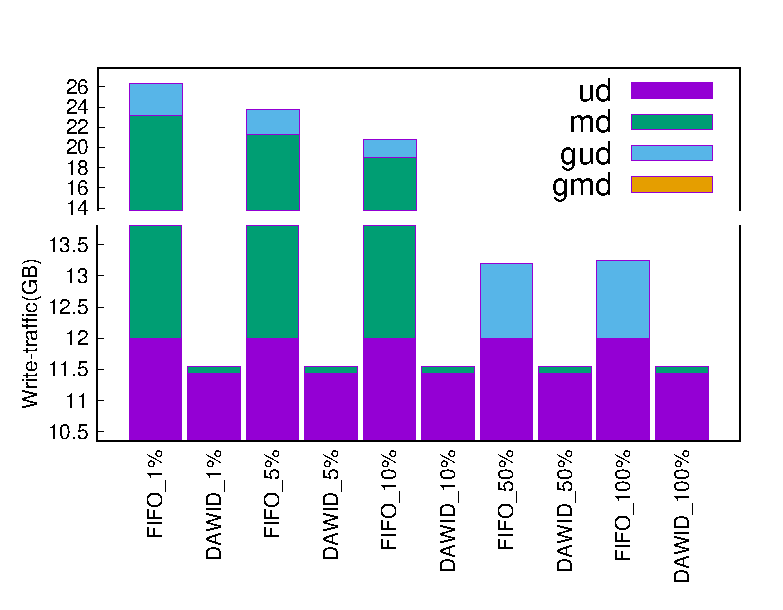
\includegraphics[width=0.3\textwidth]{expr/micro_220517/wt/result/RAND.eps}
	} 
	\subfloat[JESD] { 
	    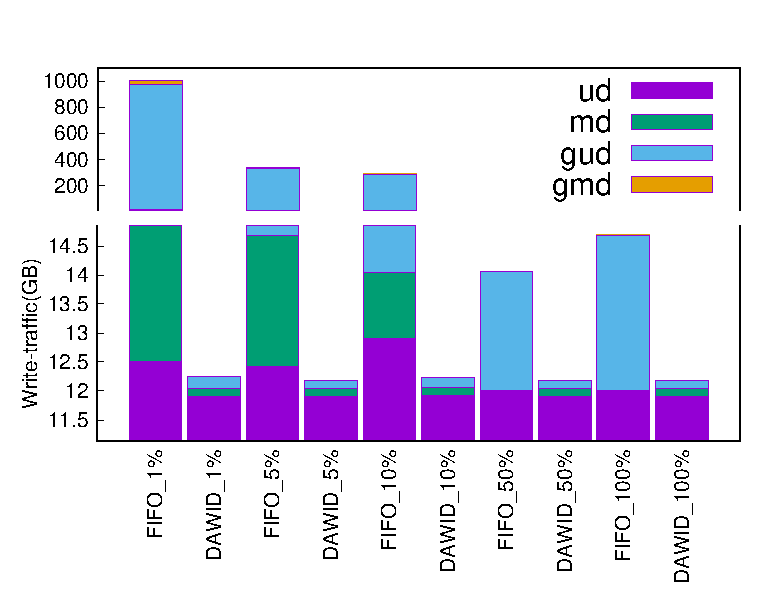
\includegraphics[width=0.3\textwidth]{expr/micro_220517/wt/result/JESD.eps}
	}
    \caption{\textbf{Write Traffic}}
\end{figure*} 


\iffalse
\begin{figure*}[t]
    \centering{}
	\subfloat[Sequential] { 
	    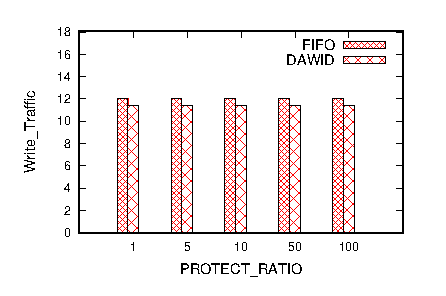
\includegraphics[width=0.3\textwidth]{expr/micro_220517/wt/perf_SEQ.eps}
	} 
	\subfloat[Random] { 
	    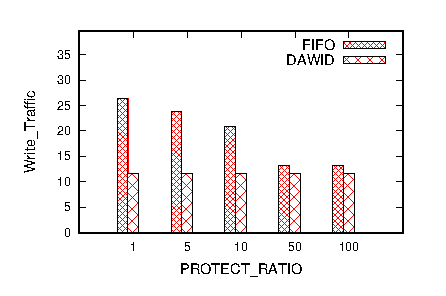
\includegraphics[width=0.3\textwidth]{expr/micro_220517/wt/perf_RAND.eps}
	} 
	\subfloat[JESD] { 
	    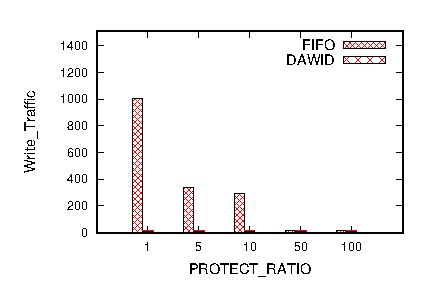
\includegraphics[width=0.3\textwidth]{expr/micro_220517/wt/perf_JESD.eps}
	}
    \caption{\textbf{Write Traffic}}
\end{figure*} 
\fi




\iffalse
%% CACHE_MISS
\begin{table}
    \centering
    \fontsize{11}{11}
    \begin{tabular}{| l | r | r | r | r | } %% KVS cache-ref cache-miss 
    \hline
    \footnotesize{\textbf{Workload}} & \footnotesize{\textbf{OPs}} & \footnotesize{\textbf{Footprint(Data)}} & \footnotesize{\textbf{Footprint(Index)}} \\ \hline \hline
    \footnotesize{sequential} & \footnotesize{2M} & \footnotesize{0,000} & \footnotesize{00,000} \\ \hline
    \footnotesize{random} & \footnotesize{2M} & \footnotesize{0,000} & \footnotesize{00,000} \\ \hline
    \footnotesize{webserver} & \footnotesize{2M} & \footnotesize{5.2G} & \footnotesize{5.8G} \\ \hline
    \footnotesize{fileserver} & \footnotesize{2M} & \footnotesize{1.9G} & \footnotesize{2.2G} \\ \hline
    \footnotesize{linkbench run} & \footnotesize{2M} & \footnotesize{5.0G} & \footnotesize{14.8G} \\ \hline
    \footnotesize{tpcc} & \footnotesize{2M} & \footnotesize{2.7G} & \footnotesize{5.8G} \\ \hline
%    \footnotesize{sequential} & \footnotesize{29,831} & \footnotesize{4,125} & \footnotesize{21,986} & \footnotesize{2,731} \\ \hline 
%    \footnotesize{random} & \footnotesize{38,272} & \footnotesize{5,810} & \footnotesize{20,949} & \footnotesize{2,727} \\ \hline 
%    \footnotesize{linkbench} & \footnotesize{9,238} & \footnotesize{4,368} & \footnotesize{4,844} & \footnotesize{1,938} \\ \hline 
%    \footnotesize{TPC-C} & \footnotesize{38,732} & \footnotesize{29,529} & \footnotesize{8,389} & \footnotesize{4,092} \\ \hline 
%    \footnotesize{Webserver} & \footnotesize{38,732} & \footnotesize{29,529} & \footnotesize{8,389} & \footnotesize{4,092} \\ \hline 
%    \footnotesize{Fileserver} & \footnotesize{38,732} & \footnotesize{29,529} & \footnotesize{8,389} & \footnotesize{4,092} \\ \hline 
    %\footnotesize{+overwrite} & \footnotesize{68,103} & \footnotesize{9,935} & \footnotesize{42,935} & \footnotesize{5,458} \\ \hline
    %\footnotesize{+readrandom} & \footnotesize{77,341} & \footnotesize{14,303} & \footnotesize{47,779} & \footnotesize{7,396} \\ \hline
    %\footnotesize{+seekrandom} & \footnotesize{116,073} & \footnotesize{43,832} & \footnotesize{56,168} & \footnotesize{11,488} \\ \hline
    \end{tabular}
    \vspace{5pt}
    \caption{\textbf{Number of cache references and misses.}
        \textbf{Ref(R)} is the number of cache references when running RocksDB; 
        \textbf{Miss(R)}, the number of cache misses with RocksDB; 
        \textbf{Ref(J)}, references with JFDB; and \textbf{Miss(J)}, misses with JFDB.
    }    
    \label{tab_cache_miss}
\end{table}
\fi 

\iffalse
\begin{figure*}[t]
    \centering{}
	\subfloat[Random Write] { 
	    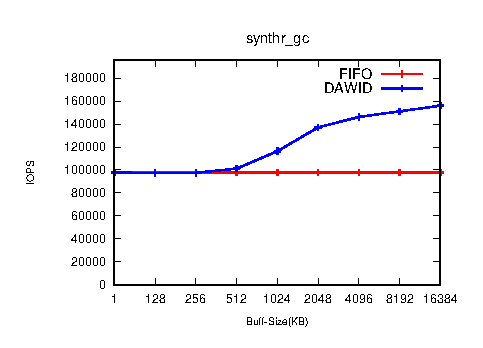
\includegraphics[width=0.3\textwidth]{expr/micro/synthr_gc.eps}
	} 
	\subfloat[Linkbench] { 
	    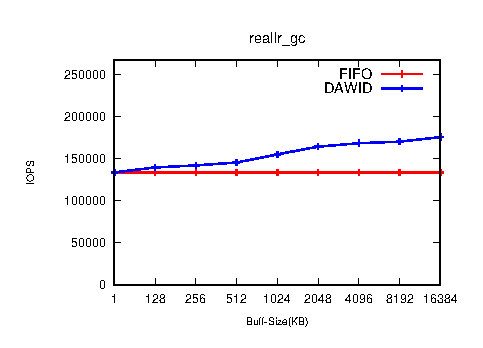
\includegraphics[width=0.3\textwidth]{expr/micro/reallr_gc.eps}
	} 
	\subfloat[TPCC] { 
	    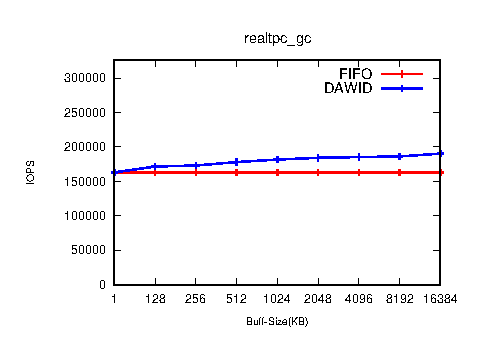
\includegraphics[width=0.3\textwidth]{expr/micro/realtpc_gc.eps}
	}
    \caption{\textbf{IOPS}}
\end{figure*} 



\begin{figure*}[t]
    \centering{}
	\subfloat[Filebench Webserver] { 
	    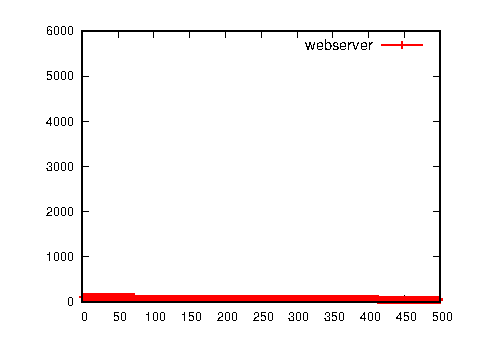
\includegraphics[width=0.4\textwidth]{webserver_uniq_500.eps}
	} 
	\subfloat[Filebench Fileserver] { 
	    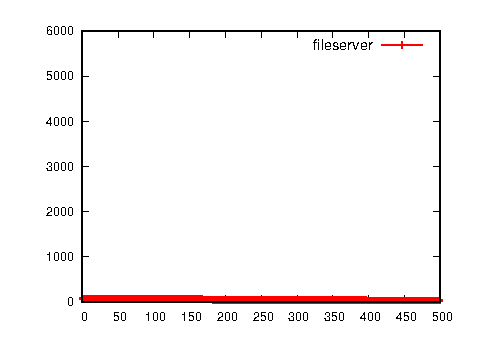
\includegraphics[width=0.4\textwidth]{fileserver_uniq_500.eps} 
	} 
    \caption{\textbf{Workload Characteristic.}}

    \centering{} 
	\subfloat[Linkbench Run] { 
	    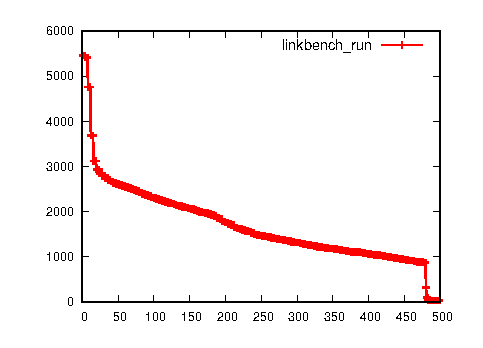
\includegraphics[width=0.4\textwidth]{linkbench_r_uniq_500.eps}
	} 
	\subfloat[TPCC] { 
	    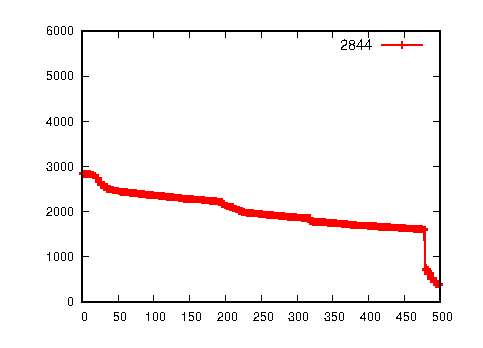
\includegraphics[width=0.4\textwidth]{tpcc_20_500.eps}
	}
    \caption{\textbf{Workload Characteristic.}}
\end{figure*} 

\fi

\subsection{Performance results}
%We assume 1\% of the mapping table is protected via capacitors in a 64GB SSD. 
%The 64GB SSD is using DRAM and assumes that 1\% of the mapping table is
%protected. 
We measured the performance of \ours{} using fio benchmark~\cite{fio-bench},
running 4KB sequential writes, 4KB random writes, and the skewed read-write
mixed workload that follows JESD219 using 8 threads.  A total of 90GB of data
was written to the 30GB area.


\begin{table}[tb]
    \centering
    \fontsize{11}{11}
    \small
	% Model Manufacturer Category PLP-Support Capacitor 
    %\begin{tabular}{p{2.4cm}|p{1.3cm}|p{1.2cm}|l}
    %\begin{tabular}{p{2.4cm}|p{2.4cm}|p{2.4cm}|p{2.4cm}|p{2.4cm}}
    \begin{tabular}{|p{5cm}|l|}
        % \hline
        % \multirow{4}{*}{{\rotatebox{90}{\parbox{1.2cm}{\centering \footnotesize{Concurrency}}}}} 
		\hline
        \bf{Data Type} &  \bf{Size} \\ \hline \hline
        % \footnotesize{\bf{Ratio}} \\ \hline \hline
	    {User Data Buffer} & {4MB} \\ \hline
		{Mapping Table} & {512MB} \\ \hline
		{Mapping Table Directory} & {512KB} \\ \hline 
% 		\footnotesize{Mapping Table Directory} & \footnotesize{128KB} & \footnotesize{0.02}\% \\ \hline
		{Metadata for Allocation} & {1MB} \\ \hline 
		{Metadata for GC(Garbage Collection)} & {9MB}  \\ \hline 
		{Total Buffer Memory} & {526.5MB} \\ \hline
% 		\footnotesize{SSD Capacity} & \footnotesize{512GB} & -  \\ \hline
    \end{tabular}
    \caption{\textbf{Components of the SSD-internal buffer.}}
    \label{tab:ssd_buff_comp}
    \vspace{-10pt}
\end{table}



\begin{table}[tb]
    \centering
    \fontsize{11}{11}
    \small
	% Model Manufacturer Category PLP-Support Capacitor 
    %\begin{tabular}{p{2.4cm}|p{1.3cm}|p{1.2cm}|l}
    %\begin{tabular}{p{2.4cm}|p{2.4cm}|p{2.4cm}|p{2.4cm}|p{2.4cm}}
    \begin{tabular}{|p{5cm}|l|}
        % \hline
        % \multirow{4}{*}{{\rotatebox{90}{\parbox{1.2cm}{\centering \footnotesize{Concurrency}}}}} 
		\hline
		\bf{Configuration} & \bf{Size} \\ \hline \hline
        Channel & 8x \\ \hline
        Way & 4x \\ \hline
        Die & 4x \\ \hline
        Plane & 4x \\ \hline
        Page Size & 4KB \\ \hline
        SSD Capacity & 512GB \\ \hline
    \end{tabular}
    \caption{\textbf{SSD Configuration.}}
    \label{tab:ssd_config}
    % \vspace{-10pt}
\end{table}
